\section{System Design}

\subsection{System Overview Diagram}

Figure \ref{fig:deployment} shows the deployment diagram for FANS. There will be three devices which communicate with
each other on a local network:

\begin{enumerate}
    \item The alarm system on a Raspberry Pi 4.
    \item The smoke detection system on a Raspberry Pi 4.
    \item A notification system on a Raspberry Pi 4.
\end{enumerate}

\begin{figure}[H]
    \centering
    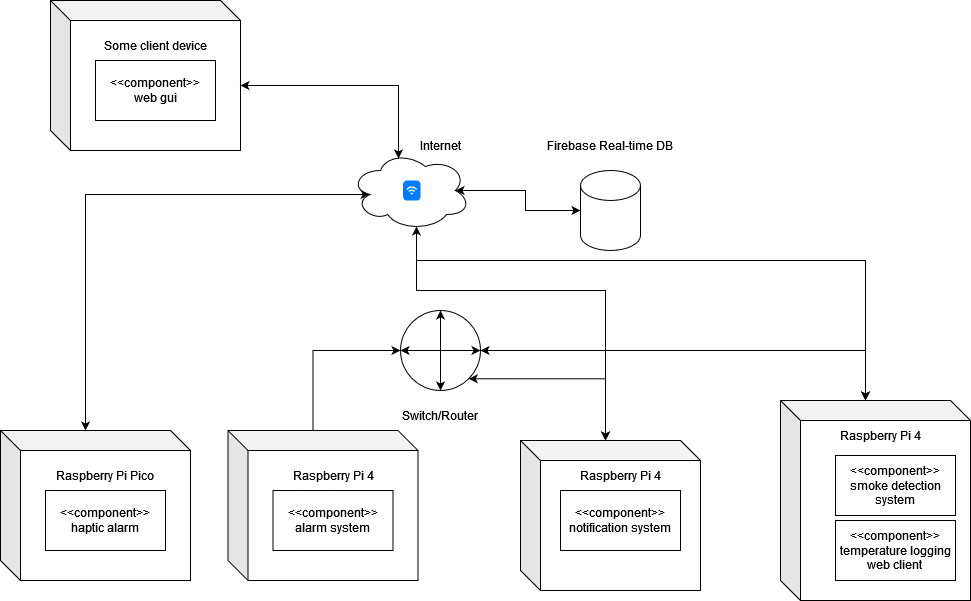
\includegraphics[width=\linewidth]{../assets/FANSDeployment.png}
    \caption{Deployment diagram of FANS.}
    \label{fig:deployment}
\end{figure}

The smoke detection and temperature logging system will continuously update the cloud database with recorded smoke and
temperature levels.

When the smoke detection system detects a smoke or temperature measurement above the limiting threshold, it will signal
the alarm system to sound the alarm using a UDP packet. It will also signal the notification system to send out
notifications to the subscriber list in the same way, and then send a write request to the cloud database to signal the
emergency detection flag.

The fourth device, the Pi Pico, will buzz when the cloud database indicates that an emergency has been detected by the
detection system. This will physically notify the user of the emergency.

The notification and alarm system are on separate devices to preserve their integrity in the case of an emergency. It
is possible that the smoke detection system will be closer to the source of the fire, and therefore be at risk of being
damaged/disabled. With the notification and alarm systems on separate devices connected through a local internet
connection, they will be able to perform their responsibilities with less risk of being damaged by flames. The local
connection also allows the alarm to sound in the case where the local network loses internet connection.

The cloud database is a real-time database to facilitate the real-time nature of display information on the web GUI. In
addition, it will allow the haptic feedback device to buzz as soon as the smoke detection system signals an emergency
to the cloud database. The fire alarm system has a real-time nature which needs to be preserved.

The web GUI will be served on the cloud, allowing us to serve our interface to multiple users more easily.

\textbf{Scalability} \\
This configuration would allow us to scale our system horizontally very easily. Multiple different alarm systems and
smoke detectors could be connected over a local network to a notification system, allowing smoke detection in multiple
rooms and alarms sounding in multiple rooms. Additionally, several haptic alarm wearable devices could be clients to
the real-time database, allowing any number of users to be notified haptically in the event of an emergency.

\textbf{Modularity} \\
Each subsystem has a single responsibility that allows for modularity in FANS. Subsystems have a clearly defined
interface with specific messages passed between them, allowing subsystems to operate without knowledge of each others’
implementations.

The smoke detection system simply sends emergency signals out over the local network to nodes who are listening, which
allows it to set off multiple alarm nodes.

The cloud database makes data available in such a way that multiple web UI clients and multiple wearable devices can
access sensor data and emergency flags.

The notification system is entirely self-contained, and only requires access to contact information in the cloud
database.

\subsubsection{Communication Protocols}

The smoke detection system will be communicating with an array of temperature and smoke sensors using the I2C protocol
over the GPIO pins of a Raspberry Pi 4.

Each node on the local network (the smoke detection system, alarm system and notification system) will communicate with
each other using UDP packets over the local network.

Nodes which communicate with the cloud hosted real-time Firebase database will use HTTP requests to interact with the
database.

\begin{itemize}
    \item The smoke detection system will post JSON payloads to the database to write data.
    \item The web GUI will request JSON over HTTP to update its visual components (dashboard with charts, etc.) with the data
          stored in the database.
    \item The notification system will request contact information from the database over HTTP to send notifications to affected
          users.
    \item The haptic alarm system will poll a database flag over HTTP to check if there is an active emergency.
\end{itemize}

Finally, the notification system will communicate with affected users over email and SMS text notifications. This will
use standard internet, SMS and email protocols.

\subsection{Component Details}

The following section will describe the interfaces and responsibilities of each major node in the FANS system.

\subsubsection{Smoke Detection System}

The first component in the proposed system is the smoke detection and temperature sensing system. It will read sensor
data from a locally connected smoke sensor and temperature sensor using the I2C protocol over the Raspberry Pi 4's GPIO
pins. It will then update the real-time Firebase database with the collected sensor data over an internet connection.

If any temperature or smoke measurements are above the critical threshold for signalling an emergency, it will send a
message to the notification system and the alarm system over UDP to signify an emergency. It will also update a flag in
the real-time database to signify that an emergency has been detected.

The smoke detection system can be configured by the user. The user configuration settings will be read from the cloud
database whenever they are updated, which allows the smoke detection system to use configurable smoke and temperature
thresholds and have a time-out.

\begin{figure}[H]
    \centering
    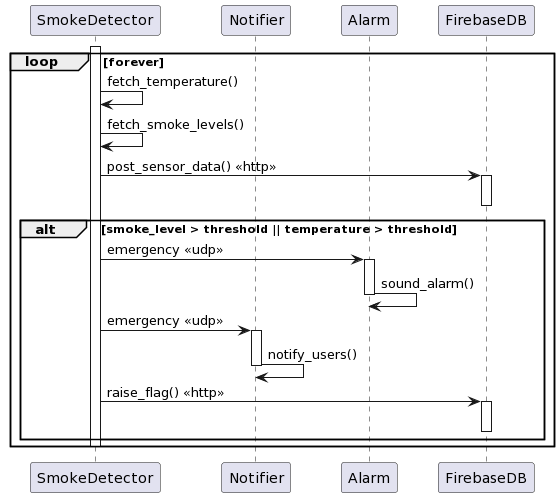
\includegraphics[width=5in]{../assets/SmokeDetectorSequence.png}
    \caption{Sequence diagram for the primary responsibilities of the smoke detector system.}
    \label{fig:smoke-detector-sq}
\end{figure}

\subsubsection{Notification System}

The notification system is responsible for notifying affected users of an emergency and triggering the alarm system. It
will also send SMS and email notifications to all users in the database to notify them of the detected emergency.

The notification system sends its notifications following the receipt of a UDP message from the smoke detection system.
The contact information of the notification recipients are stored both on its local database and the cloud database.
The local database is synchronized periodically with the cloud.

\subsubsection{Alarm System}

The alarm system is responsible for sounding an alarm in the building when an emergency has been detected. The alarm
system receives notification over UDP from the smoke detection system when an emergency has been detected, at which
point it sounds an alarm and flashes lights.

The lights will be an on-board SenseHat, and the alarm is an audio-hat module. The alarm will continue to sound until
the system receives a UDP message to stop.

\subsubsection{Haptic Alarm System}

The haptic alarm system is designed to be a wearable device that vibrates during an emergency. The device queries the
real-time database for a flag indicating an alarm. Once the flag is raised, the device vibrates until the emergency has
ended (the flag is "lowered" in the database).

\begin{figure}[H]
    \centering
    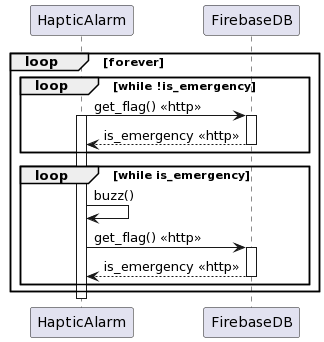
\includegraphics[width=3in]{../assets/HapticAlarmSequence.png}
    \caption{Sequence diagram for the primary responsibilities of the haptic alarm system.}
    \label{fig:haptic-alarm-sq}
\end{figure}

\subsubsection{Firebase Real-Time Database}

The real-time database is responsible for storing smoke and temperature level data in real-time, as well as a database
flag indicating emergency. User contact information will also be stored in this database. Finally, it will also contain
user-configured settings (such as smoke level threshold for triggering an emergency). It will be cloud hosted by
Firebase.

The interaction between the haptic alarm system and the real-time database is visible in Figure
\ref{fig:haptic-alarm-sq}. The interaction between the smoke detector system and the real-time database is visible in
Figure \ref{fig:smoke-detector-sq}.

\subsubsection{Web GUI}

The web GUI is responsible for displaying the sensor information from the real-time database on time-series charts. It
will also allow users to configure settings for FANS (emergency thresholds, etc.) and add more user contact information
to the notification subscriber list. It will also allow users to disable the alarm when an emergency has been resolved.

\subsection{Use Cases}

\subsubsection{Trigger Emergency}

\textbf{Flow of events}
\begin{enumerate}
    \item The smoke detection system sends a TCP message to the notification system to warn of an emergency.
    \item The smoke detection system raises a flag in the real-time database to indicate the emergency.
    \item The notification system forwards this message to the alarm system.
    \item The notification system begins sending SMS and email notifications to the users who are listed in the database.
    \item The alarm system receives the TCP message from the notification system.
    \item The alarm system sounds the alarm and flashes LEDs.
    \item The haptic alarm system reads the flag from the real-time database.
    \item The haptic alarm system begins buzzing.
\end{enumerate}

\begin{figure}[H]
    \centering
    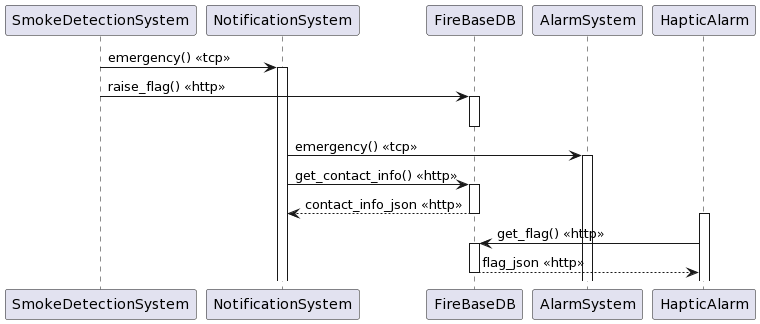
\includegraphics[width=\linewidth]{../assets/FANSAlarmUseCaseSequence.png}
    \caption{Sequence diagram for the major interactions in the "Trigger Emergency" use case.}
\end{figure}
